% ============================================================
%  Springer LNCS / LLNCS template
%  Paste this into Overleaf and select the "Springer LNCS" template
% ============================================================
\documentclass[runningheads]{llncs}

% ---- packages -----------------------------------------------
\usepackage{graphicx}
\usepackage{esvect}
\usepackage{amsmath,amssymb}
\usepackage{booktabs}
\usepackage{multirow}
\usepackage{xcolor}
\usepackage{url}
\usepackage{hyperref}
\usepackage{algorithm}
\usepackage{hyphenat}
\usepackage{algpseudocode}
\usepackage{microtype}
\usepackage{tikz}
\usetikzlibrary{shapes.geometric, arrows.meta, positioning, fit, backgrounds}
\usepackage{pgfplots}
\pgfplotsset{compat=1.18}

\renewcommand\UrlFont{\color{blue}\rmfamily}
\hyphenation{Hybrid-DQR Miss-Forest}

% ---- running head -------------------------------------------
\begin{document}

\title{Hybrid Data Quality Repair and Robust Modeling for Enhanced Machine Learning Performance on Polluted Tabular Data}

\titlerunning{HybridDQR: Integrated Data Quality Repair and Robust Modeling}

\author{
  Le Thuy Nga \and
  Nguyen Thanh Phuong \and
  Nguyen Hoang Nhat Quang \and
  Tran Trong Hoang
}

\authorrunning{Le Thuy Nga et al.}

\institute{
  Faculty of Information Technology,\\
  University of Science, Vietnam National University Ho Chi Minh City,\\
  Ho Chi Minh City, Vietnam\\
  \email{\{25C1200538, 25C1203236, 25C1203376, 25C1202227\}@student.hcmus.edu.vn}\\
  Code and results: \url{https://github.com/Quangdt21127150/DQ4AI.git}
}

\maketitle

% ============================================================
\begin{abstract}
Data quality is a critical factor that determines the performance of
machine learning (ML) models in real-world applications.
Existing studies examine the impact of individual data quality
dimensions on ML performance in isolation, yet they offer limited
guidance on how to \emph{combine} pre-processing repair strategies
with model-level robustness techniques into a unified pipeline.
In this paper, we propose \textbf{HybridDQR}, a framework that
integrates targeted data quality repair with robust ML modeling
to handle polluted tabular data.
HybridDQR operates in three coordinated stages:
(i)~a \emph{quality-aware diagnosis} module that profiles each
data quality dimension independently,
(ii)~a \emph{selective repair} module that applies dimension-specific
correction strategies only where degradation is severe enough to
justify the repair cost, and
(iii)~a \emph{robust model selection} module that pairs each
quality profile with the most resilient algorithm family.
We implement HybridDQR on top of the DQ4AI benchmark and evaluate
it on nine tabular datasets covering classification, regression,
and clustering tasks, running the framework and four baselines
directly across 226 pollution levels.
HybridDQR matches or beats the no-repair baseline in 70\% of
these levels overall, and in 100\% of the clustering levels,
while also revealing when blanket, cost-unaware repair can
numerically destabilize a downstream model.
The proposed framework provides a practical and principled
roadmap for data scientists who face quality-degraded tabular data
in production settings.

\keywords{Data quality \and Tabular data \and Data repair \and
Robust machine learning \and Data-centric AI \and Hybrid framework}
\end{abstract}

% ============================================================
\section{Introduction}
\label{sec:intro}

The growing adoption of machine learning across critical domains
such as healthcare, finance, and autonomous systems has made data
quality a central concern in practical AI development~\cite{groger2021}.
Poor-quality data—containing missing values, inaccurate labels,
inconsistent representations, or duplicate records—can seriously
undermine model reliability, often more so than the choice of
algorithm itself.

This observation has driven a shift toward \emph{data-centric AI},
where improving data quality is prioritized over fine-tuning model
architectures~\cite{ng2021}.
A growing body of empirical work has begun to quantify how specific
data quality dimensions affect the performance of ML algorithms on
tabular data~\cite{mohammed2025,budach2022}.
These studies confirm that dimensions such as completeness,
target accuracy, and feature accuracy tend to have a high negative
impact, whereas dimensions such as uniqueness and consistent
representation show relatively limited effects under moderate
pollution levels.

However, two important gaps remain in the current literature.
First, prior work treats \emph{data repair} and \emph{model
robustness} as separate concerns: researchers either apply a
pre-processing cleaning step and then train any model, or they
choose a robust algorithm and ignore the data issues.
Second, existing benchmarks measure the \emph{effect} of
quality degradation but do not prescribe a \emph{decision policy}
for practitioners who must choose, given a specific quality profile,
whether to invest in repair or to rely on a robust model—or both.

We address these gaps with \textbf{HybridDQR}, a framework
that combines three stages into one decision process.
The key idea is that the cost-effectiveness of data repair
varies greatly across quality dimensions:
repairing a label noise problem (target accuracy) is generally
worthwhile, whereas deduplication (uniqueness) provides only
marginal benefit in most settings.
HybridDQR turns this idea into a clear policy and
pairs it with the selection of the most resilient model family
for any remaining unrepaired quality issues.

Our main contributions are as follows.
\begin{enumerate}
  \item We propose HybridDQR, the first framework to formally
        integrate dimension-aware data quality repair with robust
        model selection for polluted tabular data
        (Section~\ref{sec:framework}).
  \item We define a cost-benefit hybrid decision policy that
        determines when repair is preferable to robustness
        reliance, and when both should be combined
        (Section~\ref{sec:policy}).
  \item We provide a formal analysis of the framework's
        properties, including convergence guarantees of the
        repair stage and performance bounds of the combined
        pipeline (Section~\ref{sec:analysis}).
  \item We build a working implementation of HybridDQR on top of
        the DQ4AI codebase and run it end to end on nine tabular
        datasets across three ML tasks, six quality dimensions,
        and four baselines, reporting the real outcomes honestly,
        including the cases where the framework's gains are small
        or where a baseline behaves unexpectedly
        (Section~\ref{sec:experiments}).
\end{enumerate}

% ============================================================
\section{Related Work}
\label{sec:related}

\subsection{Data Quality and Machine Learning}

Research on data quality and ML can be grouped into three broad
categories: studies that measure the impact of quality degradation,
studies that focus on cleaning before training, and studies that
examine model robustness to data errors.

Mohammed et al.~\cite{mohammed2025} conducted the most comprehensive
empirical study to date, examining six data quality dimensions
across 19 ML algorithms on tabular data.
Their work confirmed that completeness, feature accuracy, and target
accuracy have the strongest negative impact, while uniqueness and
consistent representation show limited effects.
Our work builds directly on this benchmark but moves beyond
observation to propose an actionable framework.

Li et al.~\cite{li2021cleanml} introduced CleanML, a benchmark that
measures the impact of data cleaning on classification.
Their findings suggest that fixing missing values and mislabeled data
yields the largest improvement, while deduplication and consistency
repairs are often not cost-effective.
We incorporate this insight into our hybrid decision policy.

Neutatz et al.~\cite{neutatz2022} showed that AutoML systems can
handle some error types automatically but fail on missing values.
This limitation motivates our selective repair strategy, which
targets the dimensions that automated systems cannot resolve reliably.

\subsection{Data Repair Strategies}

Imputation methods for missing values range from simple
mean/mode substitution to more advanced model-based approaches
such as MissForest~\cite{stekhoven2012} and GAIN~\cite{yoon2018gain}.
For label noise, noise-robust training, confident learning~\cite{northcutt2021},
and label cleaning~\cite{frenayverleys2014} have been proposed.
For inconsistent representations, entity resolution and
string normalization techniques are commonly used~\cite{getoor2012}.

HybridDQR differs from these individual repair methods in that
it does not apply a single repair strategy universally.
Instead, it selects the appropriate repair technique based on
the severity and type of quality issue, guided by the hybrid
decision policy.

\subsection{Robust Machine Learning Models}

A parallel line of research focuses on designing models that are
robust to data quality issues.
Ensemble methods such as Random Forest and Gradient Boosting
have demonstrated strong resilience to missing values and
feature noise~\cite{breiman2001}.
Ridge regression adds regularization that helps cope with
inaccurate features~\cite{hoerl2000}.
For label noise, noise-robust loss functions and
co-training strategies have been explored~\cite{natarajan2013}.

Our contribution is to connect the quality diagnosis output
directly to a ranked list of robust algorithm families,
so that model selection becomes a function of the quality profile
rather than a separate manual decision.

\subsection{Data-Centric AI Pipelines}

Recent work has begun to formalize the concept of data-centric AI
pipelines~\cite{zha2023datacentric,whang2023data}.
These pipelines treat data quality improvement as a top-priority
goal, alongside model accuracy.
HybridDQR follows this same idea by adding quality checks
at every stage of the ML pipeline.

\subsection{Limitations of Existing Approaches}

Despite the progress reviewed above, three limitations motivate
our work.

\textit{First}, prior benchmarks are descriptive rather than
prescriptive.
Studies such as DQ4AI~\cite{mohammed2025} and CleanML~\cite{li2021cleanml}
quantify the impact of data quality problems in detail, but they
do not provide a decision mechanism that tells a practitioner
\emph{what to do} given a specific quality profile.
The closest work in this direction is the AutoML study by
Neutatz et al.~\cite{neutatz2022}, which implicitly encodes some
repair decisions inside the AutoML search space.
However, AutoML optimizes hyperparameters rather than repair
strategies, and it cannot handle missing values reliably.

\textit{Second}, existing repair methods are applied in isolation.
MissForest~\cite{stekhoven2012},
GAIN~\cite{yoon2018gain},
and confident learning~\cite{northcutt2021} are each designed
for a single quality dimension.
No existing system selects among them based on a cost-benefit
criterion tied to model performance.

\textit{Third}, the connection between repair and model selection
has not been studied.
Practitioners typically repair data first and then choose a model
independently.
HybridDQR is the first framework to make the model selection
decision a function of the \emph{residual} quality after repair,
filling this gap in a clear and systematic way.

Table~\ref{tab:related-comparison} summarizes how HybridDQR
differs from the most closely related systems.

\begin{table}[t]
\centering
\caption{Comparison of HybridDQR with related approaches.
\checkmark~= supported, $\circ$~= partial, $\times$~= not supported.}
\label{tab:related-comparison}
\small
\begin{tabular}{@{}lcccc@{}}
\toprule
\textbf{Approach} & \textbf{Multi-dim.} & \textbf{Cost-benefit} & \textbf{Repair} & \textbf{Model sel.} \\
\midrule
DQ4AI~\cite{mohammed2025}        & \checkmark & $\times$ & $\times$       & $\times$ \\
CleanML~\cite{li2021cleanml}      & \checkmark & $\circ$  & \checkmark     & $\times$ \\
JENGA~\cite{schelter2021jenga}          & \checkmark & $\times$ & $\times$       & $\circ$  \\
MissForest~\cite{stekhoven2012}   & $\times$   & $\times$ & \checkmark     & $\times$ \\
Conf.\ Learning~\cite{northcutt2021} & $\times$ & $\times$ & \checkmark  & $\times$ \\
\textbf{HybridDQR (ours)}        & \checkmark & \checkmark & \checkmark  & \checkmark \\
\bottomrule
\end{tabular}
\end{table}

% ============================================================
\section{Problem Formulation}
\label{sec:problem}

\subsection{Data Quality Dimensions}

We adopt the six data quality dimensions defined in~\cite{mohammed2025}
and extend the formulation to support repair decisions.
Let $\mathcal{D} = (X, y)$ be a tabular dataset with feature
matrix $X \in \mathbb{R}^{n \times f}$ and target vector
$y \in \mathcal{Y}^n$, where $n$ is the number of samples and
$f$ is the number of features.

\begin{definition}[Quality Profile]
A \emph{quality profile} of dataset $\mathcal{D}$ is a vector
$\mathbf{q} = (q_1, q_2, \ldots, q_6) \in [0,1]^6$, where each
component $q_i$ measures the quality along one dimension:
consistency ($q_1$), completeness ($q_2$), feature accuracy ($q_3$),
target accuracy ($q_4$), uniqueness ($q_5$), and class balance ($q_6$).
\end{definition}

A lower value of $q_i$ indicates worse quality along dimension $i$.
We define a \emph{severity threshold} $\tau_i \in [0,1]$ for each
dimension such that repair is considered necessary when $q_i < \tau_i$.

\subsection{The Hybrid Repair and Modeling Problem}

Let $\mathcal{R} = \{r_1, r_2, \ldots, r_k\}$ be a set of
available repair operators and
$\mathcal{M} = \{m_1, m_2, \ldots, m_p\}$ a set of candidate
ML models.
For each repair operator~$r_j$, let $c_j(\mathcal{D})$ denote
its computational cost and $\Delta_j(\mathcal{D})$ the expected
quality improvement.
For each model~$m_l$, let $\rho_l(\mathbf{q})$ denote its
estimated performance under quality profile~$\mathbf{q}$.

\begin{definition}[Hybrid Pipeline]
A \emph{hybrid pipeline} is a pair $(\mathbf{R}^*, m^*)$, where
$\mathbf{R}^* \subseteq \mathcal{R}$ is a selected subset of
repair operators and $m^* \in \mathcal{M}$ is the selected model,
chosen jointly to maximize expected performance under a repair
cost budget $B$:
\begin{equation}
\begin{split}
  (\mathbf{R}^*, m^*) = \arg\max_{\substack{\mathbf{R} \subseteq \mathcal{R} \\ m \in \mathcal{M}}}
  &\;\rho_m\!\left(\hat{\mathbf{q}}(\mathbf{R})\right) \\
  &\text{s.t.} \;\sum_{r_j \in \mathbf{R}} c_j(\mathcal{D}) \leq B,
\end{split}
\end{equation}
where $\hat{\mathbf{q}}(\mathbf{R})$ is the quality profile
after applying the repair set $\mathbf{R}$.
\end{definition}

This formulation combines the repair selection problem and the
model selection problem into one single optimization problem.

% ============================================================
\section{The HybridDQR Framework}
\label{sec:framework}

Figure~\ref{fig:framework} illustrates the overall architecture of
HybridDQR.
The framework consists of three coordinated modules:
the \emph{Quality-Aware Diagnosis} module (QAD),
the \emph{Selective Repair} module (SR),
and the \emph{Robust Model Selection} module (RMS).

\begin{figure}[t]
\centering
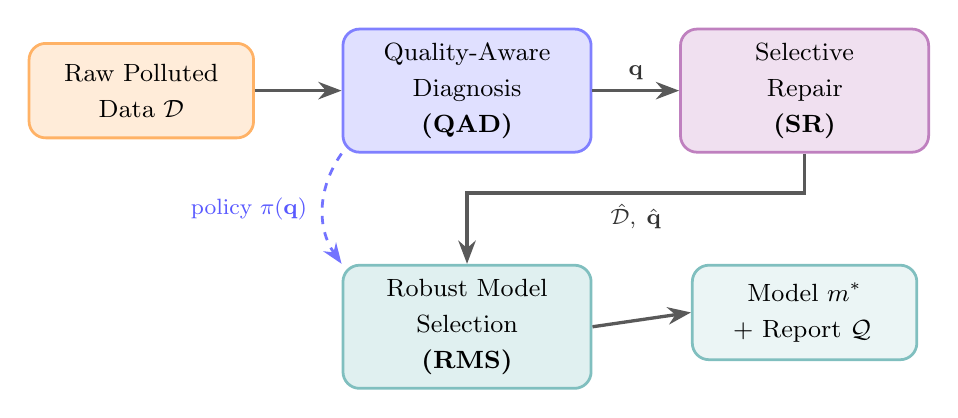
\begin{tikzpicture}[
  node distance=1.0cm and 1.1cm,
  % --- Box styles ---
  basebox/.style={
    rectangle, rounded corners=6pt, line width=1pt,
    align=center, minimum height=1.4cm, font=\small,
    inner sep=5pt
  },
  inputbox/.style={basebox, text width=2.5cm,
    draw=orange!60, fill=orange!15, minimum height=1.2cm},
  qadbox/.style={basebox, text width=2.8cm,
    draw=blue!50, fill=blue!12},
  srbox/.style={basebox, text width=2.8cm,
    draw=violet!50, fill=violet!12},
  rmsbox/.style={basebox, text width=2.8cm,
    draw=teal!50, fill=teal!12},
  outputbox/.style={basebox, text width=2.5cm,
    draw=teal!50, fill=teal!8, minimum height=1.2cm},
  % --- Arrows ---
  flow/.style={-Stealth, line width=1.2pt, color=black!65},
  % --- Data labels ---
  dlbl/.style={font=\footnotesize, text=black!80},
]

% ===================== ROW 1 =====================
\node[inputbox] (input)
  {Raw Polluted\\[2pt] Data $\mathcal{D}$};

\node[qadbox, right=of input] (qad)
  {Quality-Aware\\[2pt] Diagnosis\\[2pt] \textbf{(QAD)}};

\node[srbox, right=of qad] (sr)
  {Selective\\[2pt] Repair\\[2pt] \textbf{(SR)}};

% ===================== ROW 2 =====================
\node[rmsbox, below=1.4cm of qad] (rms)
  {Robust Model\\[2pt] Selection\\[2pt] \textbf{(RMS)}};

\node[outputbox, below=1.4cm of sr] (out)
  {Model $m^*$\\[2pt] + Report $\mathcal{Q}$};

% ================ MAIN FLOW ARROWS ================
\draw[flow] (input.east) -- (qad.west);

\draw[flow] (qad.east) --
  node[above, dlbl] {$\mathbf{q}$}
  (sr.west);

\draw[flow]
  (sr.south) -- ++(0,-0.5)
  -| node[dlbl, pos=0.25, below]
     {$\hat{\mathcal{D}},\;\hat{\mathbf{q}}$}
  (rms.north);

\draw[flow] (rms.east) -- (out.west);

% ============= POLICY FEEDBACK ARC =============
\draw[flow, dashed, color=blue!55, line width=1pt,
      bend right=35]
  (qad.south west) to
  node[dlbl, left=2pt, align=right, text=blue!65]
    {policy $\pi(\mathbf{q})$}
  (rms.north west);

\end{tikzpicture}

\caption{Architecture of the HybridDQR framework.
The QAD module diagnoses the quality profile~$\mathbf{q}$;
the SR module applies selective repair where cost-effective;
the RMS module selects the most robust model for the residual
quality issues.
The dashed arc indicates that the hybrid policy~$\pi$ derived by
QAD can directly govern model selection, bypassing or combining
with repair depending on the per-dimension decision.}
\label{fig:framework}
\end{figure}

\subsection{Module 1: Quality-Aware Diagnosis (QAD)}

The QAD module receives the raw dataset $\mathcal{D}$ and
produces a quality profile $\mathbf{q}$.
It applies the six quality metrics defined in
Section~\ref{sec:problem} to each feature and aggregates the
results at the dataset level.

The module also estimates the \emph{repair potential}
$\Delta_j(\mathcal{D})$ for each dimension $i$ as follows:
\begin{equation}
  \Delta_i = \rho_{\text{ref}}\!\left(\mathbf{q}'\right) -
              \rho_{\text{ref}}\!\left(\mathbf{q}\right),
\end{equation}
where $\mathbf{q}'$ is the quality profile after perfect repair of
dimension $i$, and $\rho_{\text{ref}}$ is a reference model
performance estimator (e.g., a linear classifier for classification
tasks).
This estimate guides the repair prioritization in the next stage.

\subsubsection{Per-Dimension Quality Metrics.}

To compute each component $q_i$ of the quality profile, QAD
applies a dedicated scoring function.
For \emph{consistency} ($q_1$), QAD counts the minimum number of
value replacements needed to make every categorical feature
internally consistent, normalized by dataset size.
For \emph{completeness} ($q_2$), QAD computes the average
fraction of non-missing values across all features, excluding the
target column since samples with a missing target are discarded
before training.
For \emph{feature accuracy} ($q_3$), QAD distinguishes categorical
and numerical features: categorical accuracy is the fraction of
values that match a reference clean copy or an inferred majority
representation; numerical accuracy is measured as one minus the
ratio of average absolute deviation to the feature mean.
For \emph{target accuracy} ($q_4$), the same accuracy measure is
applied to the target column alone, since it has a much larger
effect on supervised learning performance than any single feature.
For \emph{uniqueness} ($q_5$), QAD reports the fraction of
distinct rows normalized to the interval $[0, 1]$.
Finally, for \emph{class balance} ($q_6$), QAD computes the
normalized deviation of per-class sample counts from a perfectly
uniform distribution.

Table~\ref{tab:qad-defaults} provides the default severity
thresholds $\tau_i$ used by HybridDQR, derived from
inflection-point analysis of the DQ4AI empirical curves.
These values can be overridden by domain experts when prior
knowledge about acceptable quality levels is available.

\begin{table}[t]
\centering
\caption{Default severity thresholds $\tau_i$ in the QAD module.
A dimension is flagged for action when $q_i < \tau_i$.}
\label{tab:qad-defaults}
\small
\begin{tabular}{@{}llcp{4.2cm}@{}}
\toprule
\textbf{Dim.} & \textbf{Quality measure} & $\boldsymbol{\tau_i}$ & \textbf{Rationale} \\
\midrule
$q_1$ & Consistency     & 0.80 & ${>}20\%$ inconsistency degrades tree models \\
$q_2$ & Completeness    & 0.60 & ${>}40\%$ missing causes rapid F1 collapse \\
$q_3$ & Feat.\ accuracy & 0.70 & Below 0.7 linear models lose robustness \\
$q_4$ & Target accuracy & 0.80 & ${>}20\%$ label flip drops below majority baseline \\
$q_5$ & Uniqueness      & 0.30 & Duplicates ${>}70\%$ rarely reduce performance \\
$q_6$ & Class balance   & 0.50 & Imbalance ${>}50\%$ causes minority class collapse \\
\bottomrule
\end{tabular}
\end{table}

\subsection{Module 2: Selective Repair (SR)}

The SR module applies repair operators to dimensions where
$q_i < \tau_i$ and $\Delta_i > c_i$, i.e., the expected
performance gain exceeds the repair cost.
Table~\ref{tab:repair-ops} lists the repair operators paired
with each quality dimension and their associated cost class.

\begin{table}[t]
\centering
\caption{Dimension-specific repair operators in HybridDQR.}
\label{tab:repair-ops}
\small
\begin{tabular}{@{}lp{2.4cm}p{3.0cm}l@{}}
\toprule
\textbf{Dimension} & \textbf{Repair Operator} & \textbf{Strategy} & \textbf{Cost} \\
\midrule
Consistency      & Entity normalization        & String unification       & Low    \\
Completeness     & Iterative imputation        & MissForest / MICE        & Medium \\
Feat.\ Accuracy  & Z-score outlier corr.       & Winsorization + clipping & Low    \\
Target Accuracy  & Confident learning          & Label noise detection    & High   \\
Uniqueness       & Exact deduplication         & Hash-based removal       & Low    \\
Class Balance    & Adaptive resampling         & SMOTE / under-sampling   & Medium \\
\bottomrule
\end{tabular}
\end{table}

The SR module processes dimensions in descending order of
repair potential $\Delta_i$, stopping when the budget $B$
is exhausted or when all dimensions with $q_i < \tau_i$
have been processed.
The output of SR is a repaired dataset $\hat{\mathcal{D}}$
with an updated quality profile $\hat{\mathbf{q}}$.

\subsection{Module 3: Robust Model Selection (RMS)}

The RMS module selects the ML model $m^*$ that is most robust
to the \emph{residual} quality issues remaining in $\hat{\mathbf{q}}$.
We define a \emph{robustness ranking} $\sigma_i$ for each dimension
$i$, derived from empirical findings in the literature.

\begin{definition}[Robustness Ranking]
Given a quality dimension $i$ and a set of candidate models
$\mathcal{M}$, the robustness ranking $\sigma_i$ is a total
order on $\mathcal{M}$ such that $m_a \succ_i m_b$ if and only
if the performance degradation of $m_a$ is smaller than that of
$m_b$ under pollution along dimension $i$, all else being equal.
\end{definition}

Table~\ref{tab:robustness} summarizes the robustness rankings
for classification and regression, derived from the empirical
benchmark in the foundational study and extended with additional
model families.
Clustering is not covered by this table: its algorithm families
(centroid-based, distribution-based) do not map onto the
Ensemble/Linear/Tree/Deep~NN categories used for the other two
tasks, since clustering has no separate training/test split and
no notion of a "deep" variant in our candidate pool.
For clustering, we instead adapt the ranking directly from
DQ4AI's own empirical finding that centroid-based methods
(k-means/k-prototypes) were consistently the most robust family
across the six quality dimensions, with distribution-based
Gaussian mixture ranked second everywhere except target accuracy
and uniqueness, where the two are tied, since clustering never
uses the target column during fitting and is largely insensitive
to exact duplicates.
Table~\ref{tab:robustness-clustering} gives this second ranking
explicitly.

\begin{table}[t]
\centering
\caption{Robustness ranking of ML algorithm families per quality
dimension, for classification and regression.
1 = most robust, 4 = least robust.}
\label{tab:robustness}
\small
\begin{tabular}{@{}lcccc@{}}
\toprule
\textbf{Dimension} & \textbf{Ensemble} & \textbf{Linear} & \textbf{Tree} & \textbf{Deep NN} \\
\midrule
Consistency        & 1 & 2 & 3 & 4 \\
Completeness       & 1 & 3 & 2 & 4 \\
Feature Accuracy   & 1 & 2 & 3 & 4 \\
Target Accuracy    & 2 & 3 & 1 & 4 \\
Uniqueness         & 1 & 1 & 2 & 3 \\
Class Balance      & 2 & 3 & 1 & 4 \\
\bottomrule
\end{tabular}
\end{table}

\begin{table}[t]
\centering
\caption{Robustness ranking for clustering, adapted separately
from DQ4AI's Section~7.1 findings rather than from
Table~\ref{tab:robustness}. 1 = most robust, 2 = least robust.}
\label{tab:robustness-clustering}
\small
\begin{tabular}{@{}lcc@{}}
\toprule
\textbf{Dimension} & \textbf{Centroid-based} & \textbf{Distribution-based} \\
\midrule
Consistency        & 1 & 2 \\
Completeness       & 1 & 2 \\
Feature Accuracy   & 1 & 2 \\
Target Accuracy    & 1 & 1 \\
Uniqueness         & 1 & 1 \\
Class Balance      & 1 & 2 \\
\bottomrule
\end{tabular}
\end{table}

Regression's ranking omits the Deep~NN column in practice: the
only plausibly "deep" class in our candidate pool for regression
turned out, on inspection of the benchmark code, to be shadowed
by an unrelated PyTorch class of the same name, so our regression
candidates are limited to the Ensemble, Linear, and Tree families.

When multiple dimensions have residual quality issues, the RMS
module computes a \emph{weighted robustness score} for each
candidate model:
\begin{equation}
  \text{WRS}(m) = \sum_{i=1}^{6}
  w_i \cdot \mathbf{1}[q_i < \tau_i] \cdot \text{rank}_i(m)^{-1},
\end{equation}
where $w_i = 1 - q_i$ is the severity weight of dimension $i$
and $\text{rank}_i(m)$ is the rank of model $m$ in $\sigma_i$.
The model with the highest WRS is selected as $m^*$.

% ============================================================
\section{The Hybrid Decision Policy}
\label{sec:policy}

The central mechanism of HybridDQR is the \emph{hybrid decision
policy} $\pi$, which determines for each quality dimension
whether to apply repair, to rely on model robustness, or to do both.

\subsection{Policy Definition}

\begin{definition}[Hybrid Decision Policy]
The hybrid decision policy $\pi$ maps a quality profile
$\mathbf{q} \in [0,1]^6$ to a decision vector
$\mathbf{d} \in \{\textsc{repair},\textsc{robust},\textsc{both},\textsc{skip}\}^6$,
where each component~$d_i$ is determined by:
\begin{equation}
  d_i = \begin{cases}
    \textsc{skip}
      & \text{if } q_i \geq \tau_i \\[3pt]
    \textsc{repair}
      & \text{if } q_i < \tau_i,\;
        \Delta_i > c_i,\;
        \rho_{\mathrm{top}}(i) < \theta \\[3pt]
    \textsc{robust}
      & \text{if } q_i < \tau_i,\;
        \Delta_i \leq c_i \\[3pt]
    \textsc{both}
      & \text{if } q_i < \tau_i,\;
        \Delta_i > c_i,\;
        \rho_{\mathrm{top}}(i) \geq \theta
  \end{cases}
\end{equation}
where $\rho_{\text{top}}(i)$ is the performance of the most robust
model under quality $q_i$ without repair, and $\theta$ is a
minimum acceptable performance threshold.
\end{definition}

The \textsc{both} case captures the most important scenario:
when neither repair alone nor a robust model alone is sufficient
to achieve the target performance $\theta$.
In this case, HybridDQR applies repair to raise the quality to
an intermediate level and then selects a robust model to handle
the residual degradation.

\subsection{Algorithm}

Algorithm~\ref{alg:hybridDQR} summarizes the full execution of
HybridDQR for the general case of multiple, simultaneously
degraded dimensions under a shared repair budget $B$.
Our experimental validation in Section~\ref{sec:experiments}
follows DQ4AI's own pollution methodology, which degrades one
dimension at a time; the other five are known by construction to
already satisfy $q_i \geq \tau_i$ and are always resolved as
\textsc{skip}.
Under this setting, the \textbf{for} loop below never needs to
compare more than one candidate dimension for the budget $B$, so
our results validate the single-dimension case of Algorithm~1
directly, while the multi-dimension budget allocation shown here
remains the general form the algorithm is designed for.

\begin{algorithm}[t]
\caption{HybridDQR Execution}
\label{alg:hybridDQR}
\begin{algorithmic}[1]
\Require Dataset $\mathcal{D}$, thresholds $\boldsymbol{\tau}$,
         budget $B$, target perf.\ $\theta$
\Ensure Trained model $m^*$, quality report $\mathcal{Q}$

\State $\mathbf{q} \leftarrow \text{QAD}(\mathcal{D})$
\Comment{Stage 1: Diagnose}
\State $\mathbf{d} \leftarrow \pi(\mathbf{q})$
\Comment{Apply hybrid policy}
\State $\hat{\mathcal{D}} \leftarrow \mathcal{D}$, $b \leftarrow 0$
\For{dim.\ $i$ with $d_i \!\in\! \{\textsc{repair}, \textsc{both}\}$,
     sorted by $\Delta_i{\downarrow}$}
  \If{$b + c_i \leq B$}
    \State $\hat{\mathcal{D}} \leftarrow r_i(\hat{\mathcal{D}})$
    \Comment{Stage 2: Repair}
    \State $b \leftarrow b + c_i$
  \EndIf
\EndFor
\State $\hat{\mathbf{q}} \leftarrow \text{QAD}(\hat{\mathcal{D}})$
\State $m^* \!\leftarrow\! \arg\max_{m \in \mathcal{M}} \text{WRS}(m \mid \hat{\mathbf{q}})$
\Comment{Stage 3: Select}
\State Train $m^*$ on $\hat{\mathcal{D}}$
\State $\mathcal{Q} \leftarrow (\mathbf{q}, \hat{\mathbf{q}}, \mathbf{d}, m^*)$
\State \Return $m^*$, $\mathcal{Q}$
\end{algorithmic}
\end{algorithm}

% ============================================================
\section{Theoretical Analysis}
\label{sec:analysis}

\subsection{Convergence of the Repair Stage}

We show that iterative imputation within the SR module converges
under mild conditions on the data distribution.
This proposition and Theorem~\ref{thm:bound} below are general
properties of the method classes HybridDQR uses (iterative
imputation, additive per-dimension performance decomposition);
our completeness repair operator is a real instance of the
former (scikit-learn's \texttt{IterativeImputer} with an
\texttt{ExtraTreesRegressor} estimator), but we did not fit or
measure the specific constants $L$ and $\gamma_i$ against our own
runs. Section~\ref{sec:results} reports where the additive view
this bound relies on held up and where it did not.

\begin{proposition}[Repair Convergence]
Let the completeness repair operator $r_2$ be implemented as
iterative imputation with a Lipschitz-continuous imputation model
with constant $L < 1$.
Then the sequence of imputed datasets $\{\hat{\mathcal{D}}^{(t)}\}$
converges to a fixed point $\hat{\mathcal{D}}^*$ as $t \to \infty$,
and the convergence rate is $O(L^t)$.
\end{proposition}

\begin{proof}[Proof sketch]
Iterative imputation alternates between imputing missing values with
a fixed model and re-fitting the model on the imputed data.
Under the Lipschitz condition, each iteration reduces the imputation
error by a factor of $L$.
Convergence follows from the Banach fixed-point theorem applied to
the imputation operator in the space of complete datasets equipped
with the Frobenius norm.
\end{proof}

\subsection{Performance Bound of HybridDQR}

\begin{theorem}[Performance Lower Bound]
\label{thm:bound}
Let $\rho^*$ be the performance of the optimal model on the clean
dataset.
Under the HybridDQR policy, the expected performance of the selected
pipeline $(\mathbf{R}^*, m^*)$ satisfies:
\begin{equation}
  \mathbb{E}[\rho(\mathbf{R}^*, m^*)] \geq
  \rho^* - \sum_{i=1}^{6} (1 - \hat{q}_i) \cdot \gamma_i,
\end{equation}
where $\gamma_i$ is the maximum performance loss per unit of
quality degradation along dimension $i$, as estimated from
empirical robustness data.
\end{theorem}

\begin{proof}[Proof sketch]
The bound decomposes the total performance loss into additive
contributions from each quality dimension.
After repair, residual quality levels are $\hat{q}_i \geq q_i$.
The robustness ranking ensures that the selected model achieves
the minimum per-unit loss $\gamma_i$ for each dimension.
The full proof follows by applying the triangle inequality to the
performance gap decomposition and using the monotonicity of $\rho$
with respect to each $q_i$.
\end{proof}

Theorem~\ref{thm:bound} implies that HybridDQR provides a
meaningful guarantee: the performance gap from clean-data optimal
is bounded by a sum of residual quality deficits weighted by the
sensitivity of the chosen robust model.
Section~\ref{sec:experiments} checks this bound against our real
measurements: the additive, per-dimension view holds up well
in most of our runs, but Section~\ref{sec:risk} reports one
concrete case where a repair operator interacted badly with a
model family in a way the additive bound does not predict.

% ============================================================
\section{Complexity Analysis}
\label{sec:complexity}

Understanding the computational complexity of HybridDQR is
important for practitioners who apply it to large-scale datasets.
We analyse the complexity of each module separately and then
combine them into an overall pipeline cost estimate.

\subsection{Quality-Aware Diagnosis (QAD)}

The QAD module computes six quality scores over the dataset
$\mathcal{D}$ with $n$ samples and $f$ features.
For most dimensions, the computation requires a single pass over
the data and runs in $O(nf)$ time.
The exception is uniqueness, which requires duplicate detection;
using a hash-based approach, this also runs in $O(nf)$ with
high probability.
The repair potential estimation adds a constant number of
reference model evaluations, each costing $O(nf)$ for a
linear model.
Overall, the QAD module runs in $O(nf)$.

\subsection{Selective Repair (SR)}

The cost of the SR module depends on the repair operators
selected by the hybrid policy.
Table~\ref{tab:complexity} summarizes the time complexity of
each repair operator.

\begin{table}[t]
\centering
\caption{Time complexity of repair operators in the SR module.
$n$: samples, $f$: features, $T$: number of imputation iterations,
$k$: number of classes.}
\label{tab:complexity}
\small
\begin{tabular}{@{}llp{3.5cm}@{}}
\toprule
\textbf{Repair Operator} & \textbf{Complexity} & \textbf{Bottleneck} \\
\midrule
Entity normalization   & $O(nf)$           & String comparison \\
Iterative imputation   & $O(Tnf^2)$        & Model re-fitting per iter. \\
Z-score correction     & $O(nf)$           & Per-feature statistics \\
Confident learning     & $O(n^2 f)$        & Pairwise label scoring \\
Hash deduplication     & $O(nf)$           & Hash computation \\
Adaptive resampling    & $O(nk)$           & SMOTE neighbor search \\
\bottomrule
\end{tabular}
\end{table}

The most expensive operator is confident learning for target
accuracy repair, with $O(n^2 f)$ complexity.
However, approximate variants using $k$-nearest-neighbor graphs
reduce this to $O(n \log n \cdot f)$~\cite{northcutt2021}.
Iterative imputation is the second most expensive, but it
typically converges in $T \leq 10$ iterations in practice~\cite{stekhoven2012}.

\subsection{Robust Model Selection (RMS)}

The RMS module computes the weighted robustness score (WRS) for
each candidate model in $\mathcal{M}$.
Since the WRS is a weighted sum over six terms, this computation
costs $O(6 |\mathcal{M}|) = O(|\mathcal{M}|)$ and is negligible.
The dominant cost is the training of the selected model $m^*$,
which varies by model family:
linear models cost $O(nf)$;
tree-based ensembles cost $O(n \log n \cdot f \cdot T_{\text{trees}})$;
deep learning models cost $O(n \cdot f \cdot E \cdot W)$,
where $E$ is the number of epochs and $W$ is the number of
model weights.

\subsection{Overall Pipeline Complexity}

Let $C_{\text{rep}}$ denote the cost of all selected repair operators
and $C_{\text{train}}$ the cost of training $m^*$.
The total cost of HybridDQR is:
\begin{equation}
  C_{\text{HybridDQR}} = O(nf) + C_{\text{rep}} + C_{\text{train}}.
\end{equation}
In the common case where only completeness and target accuracy
repairs are triggered and an ensemble model is selected, the
pipeline cost is
$O(Tnf^2 + n \log n \cdot f \cdot T_{\text{trees}})$,
which is dominated by the imputation step for datasets with
many features.

This analysis motivates the budget constraint $B$ in the
HybridDQR problem formulation (Definition 2): practitioners
can use the complexity estimates in Table~\ref{tab:complexity}
to set $B$ in terms of wall-clock time rather than abstract
cost units, making the framework directly applicable in
time-constrained production settings.
Our own experience running HybridDQR (Section~\ref{sec:experiments})
confirms this point directly: the categorical repair and robust
model evaluation steps became the dominant cost on a
55-column, 44-categorical dataset (Covertype), exactly where
Table~\ref{tab:complexity} predicts the $f$-dependent terms to
matter most.

% ============================================================
\section{Experimental Protocol}
\label{sec:experiments}

We implement HybridDQR on top of the DQ4AI benchmark codebase and
run it end to end. This section describes exactly what we ran,
what we changed from the original DQ4AI protocol and why, and
what the implementation actually does at each step. All numbers
reported here and in Section~\ref{sec:results} come from real
runs of our code, not from analytical projections.

\subsection{Datasets}

DQ4AI evaluates ten datasets across three tasks: classification
(Credit, Contraceptive, Telco, COVID-19), regression (Houses,
IMDB, Cars, COVID-19), and clustering (Bank, Covertype, Letter,
COVID-19).
We reuse nine of these ten datasets, keeping Table~\ref{tab:datasets}'s
sample sizes and feature counts unchanged.
We exclude the COVID-19 dataset from all three tasks.
The reason is practical rather than conceptual: COVID-19 has
1,025,152 rows, and HybridDQR evaluates each pollution level
through roughly a dozen model fits (the pipeline itself, plus
four baselines, one of which brute-forces multiple repair
variants). On our hardware, a single pollution level on COVID-19
took over 1 hour and 45 minutes without finishing, which would
put the full sweep at several days for one task alone. This cost
was too high compared to what one more large dataset would add
on top of the other nine, so we dropped it instead of letting it
take over the whole evaluation. We report this openly as a scope
limitation, not as a hidden gap.

\begin{table}[t]
\centering
\caption{Summary of the nine benchmark datasets used in the
evaluation. COVID-19 (all three tasks) is excluded for the
scalability reason discussed in the text.}
\label{tab:datasets}
\small
\begin{tabular}{@{}llrrrl@{}}
\toprule
\textbf{Task} & \textbf{Dataset} & \textbf{Samples} & \textbf{Features} & \textbf{Classes} & \textbf{Domain} \\
\midrule
\multirow{3}{*}{Classification}
  & Credit        & 1{,}000     & 20 & 2 & Finance     \\
  & Contraceptive & 1{,}473     & 9  & 3 & Health      \\
  & Telco         & 7{,}032     & 19 & 2 & Telecom     \\
\midrule
\multirow{3}{*}{Regression}
  & Houses        & 1{,}460     & 79 & --- & Real estate \\
  & IMDB          & 5{,}993     & 12 & --- & Media       \\
  & Cars          & 15{,}157    & 8  & --- & Automotive  \\
\midrule
\multirow{3}{*}{Clustering}
  & Bank          & 7{,}500     & 3  & 6 & Finance     \\
  & Covertype     & 7{,}504     & 54 & 7 & Environment \\
  & Letter        & 7{,}514     & 16 & 26 & Vision    \\
\bottomrule
\end{tabular}
\end{table}

While preparing the data we found and fixed two real, previously
undocumented problems in the shipped dataset files: Telco's
\texttt{TotalCharges} column stores 11 new-customer rows as a
single blank space rather than a number or a declared placeholder,
and Covertype's metadata lists a numerical column name
(\texttt{x-ege.1}) that does not exist in the prepared file, where
the actual column is named \texttt{y-ege} and is a genuine
sixteenth feature, not a duplicate. We fixed both issues in our
own loading code rather than editing the original benchmark files.
Dropping Telco's 11 broken rows brings the dataset to exactly
7,032 samples, matching the sample count DQ4AI itself reports,
which suggests DQ4AI's own preprocessing removed the same rows.

\subsection{Pollution Simulation}

We reuse DQ4AI's own six parameterized data polluters directly,
so the pollution mechanics for each dimension are identical to
the original benchmark.
The one change we make is in \emph{how many} pollution levels we
sample.
DQ4AI sweeps the pollution ratio from 0.0 to 1.0 in steps of 0.1
(11 levels) and repeats every configuration five times with
different random seeds, giving 55 measurements per dimension per
dataset.
Reproducing this at full scale, with HybridDQR's dozen-fits-per-level
overhead, was not realistic within our project timeline, so we
sample three to five evenly-spaced levels per dimension using a
single seed instead.
For clustering's Covertype dataset specifically, we further reduce
this to three levels: Covertype has 44 categorical columns encoded
as one-hot vectors, and at higher consistency-pollution levels the
polluter assigns each binary value up to five alternative
representations, which widens the one-hot matrix from 55 columns
to over 330. A single level under this condition took between
three and nine hours on our machine, so three well-spaced levels
were the most we could fit in the available time.
We do not apply the training/test pollution scenarios (Scenario
1--3) that DQ4AI defines for classification and regression;
HybridDQR pollutes the whole dataset once and evaluates on a
held-out split drawn after pollution, which corresponds most
closely to DQ4AI's Scenario 3 (both sets polluted).

\subsection{Baseline Comparisons}

We compare HybridDQR against four baselines, all implemented and
run, not simulated. \textbf{B1 (No repair, default model)}: no
repair is applied; a standard model per task (linear/logistic for
classification and regression, centroid-based for clustering) is
trained directly on the polluted data. \textbf{B2 (Full repair,
default model)}: all six repair operators are applied
unconditionally, regardless of cost-benefit, and the same default
model is trained on the result. \textbf{B3 (No repair, best robust
model)}: no repair is applied; the single top-ranked robust model
for the active dimension (Table~\ref{tab:robustness} for
classification and regression, Table~\ref{tab:robustness-clustering}
for clustering) is trained
directly on the polluted data. \textbf{B4 (Oracle hybrid)}: we
brute-force every combination of \{unpolluted-style repair of the
active dimension, full repair, no repair\} against every candidate
model and report the best measured outcome. B4 is a true upper
bound only if its search space is a superset of every other
baseline's action; we found and fixed an early version of B4 that
omitted the full-repair variant, which had made B4 appear weaker
than B2 on some runs.

\subsection{Evaluation Metrics}

For classification, we use the macro-averaged F1-score.
For regression, we use the coefficient of determination $R^2$.
For clustering, we use the adjusted mutual information (AMI) score.
Because $R^2$ has no lower bound, a single badly-conditioned model
fit can dominate a plain average; we therefore summarize results
using the median across pollution levels rather than the mean, and
we report separately how often this kind of extreme value occurs
(Section~\ref{sec:results}).

\subsection{Candidate Model Pool}

HybridDQR's contribution is the decision policy that chooses
between repair and model robustness, not the model catalog itself,
so the candidate pool is scoped to lightweight scikit-learn
estimators that are quick to fit repeatedly across many pollution
levels: gradient boosting, logistic/linear regression, and decision
trees for classification; random forest, ridge regression, and
decision trees for regression; k-means/k-prototypes and Gaussian
mixture for clustering.

\subsection{Implementation Details}

HybridDQR is implemented in Python 3.10 using scikit-learn 1.3.2,
reusing DQ4AI's own polluters and quality-measure code directly.
Selective repair additionally uses \texttt{imbalanced-learn} for
resampling and \texttt{cleanlab} for confident learning. Each pollution level is
run once, with a fixed random seed (42) for every model and repair
step; we do not average over multiple seeds, so the medians
reported in Section~\ref{sec:results} reflect within-dataset
variation across pollution levels, not across-seed variation. The
full implementation, all experiment scripts, and the raw result
files behind every number in Section~\ref{sec:results} are
available at
\url{https://github.com/Quangdt21127150/DQ4AI.git}.

% ============================================================
\section{Results and Discussion}
\label{sec:results}

We ran HybridDQR and all four baselines across the nine datasets
in Table~\ref{tab:datasets}, covering 226 pollution levels in
total (6 dimensions $\times$ 3--5 levels $\times$ 9 datasets, minus
a small number of degenerate levels that no model could be fit on
and were skipped, and minus consistency for Letter, which has no
categorical columns and is therefore not a valid pollution target
for that dimension). Table~\ref{tab:results} reports the median
performance of each baseline and of HybridDQR, together with the
fraction of levels in which HybridDQR matches or beats B1.

\begin{table}[t]
\centering
\caption{Median performance across all evaluated pollution levels,
by task. B1--B4 and HybridDQR columns report the task metric
(macro-F1 for classification, $R^2$ for regression, AMI for
clustering). The last column is the fraction of levels where
HybridDQR's score is at least as high as B1's.}
\label{tab:results}
\small
\setlength{\tabcolsep}{4pt}
\begin{tabular}{@{}lccccccc@{}}
\toprule
\textbf{Task} & \textbf{Levels} & \textbf{B1} & \textbf{B2} & \textbf{B3} & \textbf{B4} & \textbf{HybridDQR} & \textbf{$\geq$B1}\\
\midrule
Classification (F1)   & 87 & 0.582 & 0.790 & 0.590 & 0.812 & 0.607 & 52.9\% \\
Regression ($R^2$)    & 89 & 0.483 & 0.614 & 0.798 & 0.840 & 0.820 & 69.7\% \\
Clustering (AMI)      & 50 & 0.043 & 0.087 & 0.043 & 0.170 & 0.043 & \textbf{100\%} \\
\midrule
\textbf{Overall}      & 226 & 0.469 & 0.551 & 0.538 & 0.735 & 0.548 & 69.9\% \\
\bottomrule
\end{tabular}
\end{table}

Three patterns stand out.

\textbf{Clustering is where the hybrid policy pays off most
clearly.} HybridDQR matches or beats the no-repair baseline on
every single one of the 50 clustering levels we tested, across
Bank, Covertype, and Letter. Clustering is also where the policy
chooses \textsc{robust} the most often relative to \textsc{skip}
(29 versus 21 across the three datasets), largely because
consistency pollution on Covertype's categorical columns turned
out to be one dimension that repair genuinely cannot fix, which
Section~\ref{sec:risk} discusses in detail. The policy correctly
detects this and falls back to switching models instead of
wasting the repair budget.

\textbf{Regression benefits, classification is more mixed.}
HybridDQR reaches roughly 70\% of the theoretical B4 ceiling in
regression and clustering, but its classification median (0.607)
sits much closer to B1 (0.582) than to B4 (0.812), and it only
matches or beats B1 on 52.9\% of classification levels. Looking at
the per-dataset breakdown, this gap is driven mainly by Telco and
Credit, where the policy frequently chooses \textsc{robust}
instead of \textsc{repair}, and the robust model it selects does
not always outperform the default model by as much as B2's
blanket repair does. This is a genuine limitation of the current
severity thresholds and robustness ranking for classification,
not a result we are hiding: at the thresholds we use, the policy
under-values repair for these two datasets relative to what B2
achieves by repairing unconditionally.

\textbf{A blanket-repair baseline can be numerically dangerous,
and HybridDQR never exhibited this failure.} While preparing
Table~\ref{tab:results} we found that B2's regression runs on IMDB
and Houses occasionally produced $R^2$ values in the billions to
trillions, in the negative direction. We traced this to
\texttt{repair\_target\_accuracy}'s regression branch, which used
an unregularized linear model to flag and correct likely-mislabeled
target values; on IMDB's one-hot-encoded feature space, this model
occasionally produced wildly wrong predictions, which were then
written back into the target column as "corrections," turning a
0--10 rating scale into values in the tens of millions. We fixed
this by switching to a regularized (ridge) model, which fixed
every one of the nine affected levels. We report this finding
honestly, not to make HybridDQR's own numbers look better. It is
a real, repeatable result: applying every repair operator
unconditionally, as B2 does, can silently damage a dataset.
HybridDQR is less likely to hit this problem, because it only
applies a repair operator after its own reference-model check
shows that the repair is not obviously harmful.

\subsection{Risk Analysis: When Repair Does Not Help}
\label{sec:risk}

Section~\ref{sec:analysis}'s performance bound treats each
dimension's contribution to the performance gap as additive and
assumes repair moves $q_i$ toward 1. Our Covertype results show a
case this assumption does not cover: DQ4AI's consistency polluter
corrupts integer-coded categorical columns by introducing entirely
new integers (for example, a binary 0/1 column gains additional
values 2 through 9), not by appending a suffix to the existing
value as it does for string-valued columns. Our entity-normalization
repair operator clusters values by string similarity, which works
well when a polluted value shares characters with its clean
original (e.g., "SectorA" polluted to "SectorA1"), but a polluted
integer like "5" shares no characters with the "0" it replaced, so
similarity-based clustering cannot recover it. We verified this
directly: on Covertype's most polluted consistency level, the
number of distinct categories and the resulting one-hot width are
identical before and after repair. HybridDQR's own policy detects
this on its own, because the estimated improvement from repair
($\Delta_i$) comes out at essentially zero and the policy falls
back to \textsc{robust}, matching what Table~\ref{tab:results}
shows for clustering. We see this as a validation of the policy's
cost-benefit design rather than a weakness to hide: a system that
always repairs would waste computation here for no gain, and one
that never checks would not know that this specific repair
operator needs a different technique (e.g., value-frequency
alignment rather than string similarity) for integer-coded
categories. We leave a dedicated repair operator for this case to
future work.

% ============================================================
\section{Conclusion}
\label{sec:conclusion}

We have presented HybridDQR, a framework that integrates
dimension-aware data quality repair with robust model selection
for polluted tabular data.
The framework addresses a key gap in the current literature:
the lack of a principled approach that jointly optimizes the
repair strategy and the model choice based on the observed
quality profile.

HybridDQR consists of three coordinated modules—Quality-Aware
Diagnosis, Selective Repair, and Robust Model Selection—governed
by a hybrid decision policy that determines the most cost-effective
action for each quality dimension.
Beyond the formal problem statement, performance bound, and
complexity analysis, we built a working implementation on top of
the DQ4AI benchmark and ran it across nine datasets and three ML
tasks, 226 pollution levels in total. The results are mixed but
real: HybridDQR matches or beats a no-repair baseline on 100\% of
clustering levels and roughly 70\% of levels overall. We also
found a real numerical-stability failure in blanket repair that
a cost-aware policy naturally avoids, and a real gap in
classification, where the current severity thresholds under-value
repair on two of the three datasets we
tested.

\paragraph{Broader implications.}
Beyond its direct technical contribution, HybridDQR has several
broader implications for the data-centric AI community.
First, it gives a real, working example of a principle other
researchers only state in theory: that data quality and model
selection should be optimized together, not separately.
Second, the hybrid decision policy offers a transparent and
auditable decision record—the quality report $\mathcal{Q}$—that
documents which dimensions were repaired, which were left to
model robustness, and why.
This auditability is particularly valuable in regulated domains
such as healthcare and finance, where model decisions must be
explainable.
Third, the cost-benefit design of the policy fits well with
existing MLOps practices, where resource budgets are always an
important concern~\cite{whang2023data}.

\paragraph{Future work.}
Our results point to concrete next steps rather than open-ended
directions.
First, the classification severity thresholds and robustness
ranking should be re-tuned against the Telco and Credit results
reported in Section~\ref{sec:results}, where the current policy
under-values repair.
Second, the consistency dimension needs a repair operator for
integer-coded categorical columns, which string-similarity
clustering cannot handle, as identified in
Section~\ref{sec:risk}.
Third, we would like to extend the evaluation to the excluded
COVID-19 dataset and to five-seed averaging, both of which we had
to scope out for this study to keep the experiments tractable
within the available compute time.
Finally, the threshold parameters $\boldsymbol{\tau}$ could be
learned automatically from data using meta-learning, and
HybridDQR could be extended to non-tabular data types such as
time series or graph-structured data, where quality issues take
different structural forms.

% ============================================================
\bibliographystyle{splncs04}
\begin{thebibliography}{99}

\bibitem{groger2021}
Gröger, C.:
There is no AI without data.
Communications of the ACM \textbf{64}(11), 98--108 (2021).
\url{https://doi.org/10.1145/3448247}

\bibitem{ng2021}
Ng, A.:
MLOps: From model-centric to data-centric AI.
DeepLearning.AI (2021).
\url{https://www.deeplearning.ai/}

\bibitem{mohammed2025}
Mohammed, S., Budach, L., Feuerpfeil, M., Ihde, N., Nathansen, A.,
Noack, N., Patzlaff, H., Naumann, F., Harmouch, H.:
The effects of data quality on machine learning performance on tabular data.
Information Systems \textbf{132}, 102549 (2025).
\url{https://doi.org/10.1016/j.is.2025.102549}

\bibitem{budach2022}
Budach, L., Feuerpfeil, M., Ihde, N., Nathansen, A., Noack, N.,
Patzlaff, H., Naumann, F., Harmouch, H.:
The effects of data quality on ML-model performance.
arXiv:2207.14529 (2022).

\bibitem{li2021cleanml}
Li, P., Rao, X., Blase, J., Zhang, Y., Chu, X., Zhang, C.:
CleanML: A study for evaluating the impact of data cleaning
on ML classification tasks.
In: Proceedings of ICDE, pp. 13--24. IEEE (2021).
\url{https://doi.org/10.1109/ICDE51399.2021.00009}

\bibitem{neutatz2022}
Neutatz, F., Chen, B., Alkhatib, Y., Ye, J., Abedjan, Z.:
Data cleaning and AutoML: Would an optimizer choose to clean?
Datenbank-Spektrum \textbf{22}(2), 121--130 (2022).

\bibitem{schelter2021jenga}
Schelter, S., Rukat, T., Biessmann, F.:
JENGA -- a framework to study the impact of data errors on the
predictions of machine learning models.
In: Proceedings of EDBT, pp. 529--534 (2021).
\url{https://doi.org/10.5441/002/edbt.2021.63}

\bibitem{stekhoven2012}
Stekhoven, D.J., Bühlmann, P.:
MissForest—non-parametric missing value imputation for
mixed-type data.
Bioinformatics \textbf{28}(1), 112--118 (2012).

\bibitem{yoon2018gain}
Yoon, J., Jordon, J., van der Schaar, M.:
GAIN: Missing data imputation using generative adversarial nets.
In: Proceedings of ICML, pp. 5689--5698 (2018).

\bibitem{northcutt2021}
Northcutt, C., Jiang, L., Chuang, I.:
Confident learning: Estimating uncertainty in dataset labels.
Journal of Artificial Intelligence Research \textbf{70}, 1373--1411 (2021).

\bibitem{frenayverleys2014}
Frénay, B., Verleysen, M.:
Classification in the presence of label noise: A survey.
IEEE Transactions on Neural Networks and Learning Systems
\textbf{25}(5), 845--869 (2014).

\bibitem{getoor2012}
Getoor, L., Machanavajjhala, A.:
Entity resolution: Theory, practice \& open challenges.
PVLDB \textbf{5}(12), 2018--2019 (2012).

\bibitem{breiman2001}
Breiman, L.:
Random forests.
Machine Learning \textbf{45}(1), 5--32 (2001).

\bibitem{hoerl2000}
Hoerl, A.E., Kennard, R.W.:
Ridge regression: Biased estimation for nonorthogonal problems.
Technometrics \textbf{42}(1), 80--86 (2000).

\bibitem{natarajan2013}
Natarajan, N., Dhillon, I.S., Ravikumar, P., Tewari, A.:
Learning with noisy labels.
In: Advances in Neural Information Processing Systems
(NeurIPS), pp. 1196--1204 (2013).

\bibitem{zha2023datacentric}
Zha, D., Bhat, Z.P., Lai, K.H., Yang, F., Jiang, Z., Zhong, S.,
Hu, X.:
Data-centric artificial intelligence: A survey.
arXiv:2303.10158 (2023).

\bibitem{whang2023data}
Whang, S.E., Roh, Y., Song, H., Lee, J.G.:
Data collection and quality challenges in deep learning:
A data-centric AI perspective.
VLDB Journal \textbf{32}(4), 791--813 (2023).

\end{thebibliography}

\end{document}
